\chapter{Base Experiment}
\label{ch:Base_Experiment}

This chapter describes the base experiment, which serves the purpose of applying the approach and probing the hypothesis, presented in Chapter \ref{ch:Methodology}. A summarized representation of the workflow can be seen in Fig. \ref{fig:base_workflow}. In the following, we outline the steps for executing the experiment and the results of the evaluation.

\begin{figure}
  \centering
  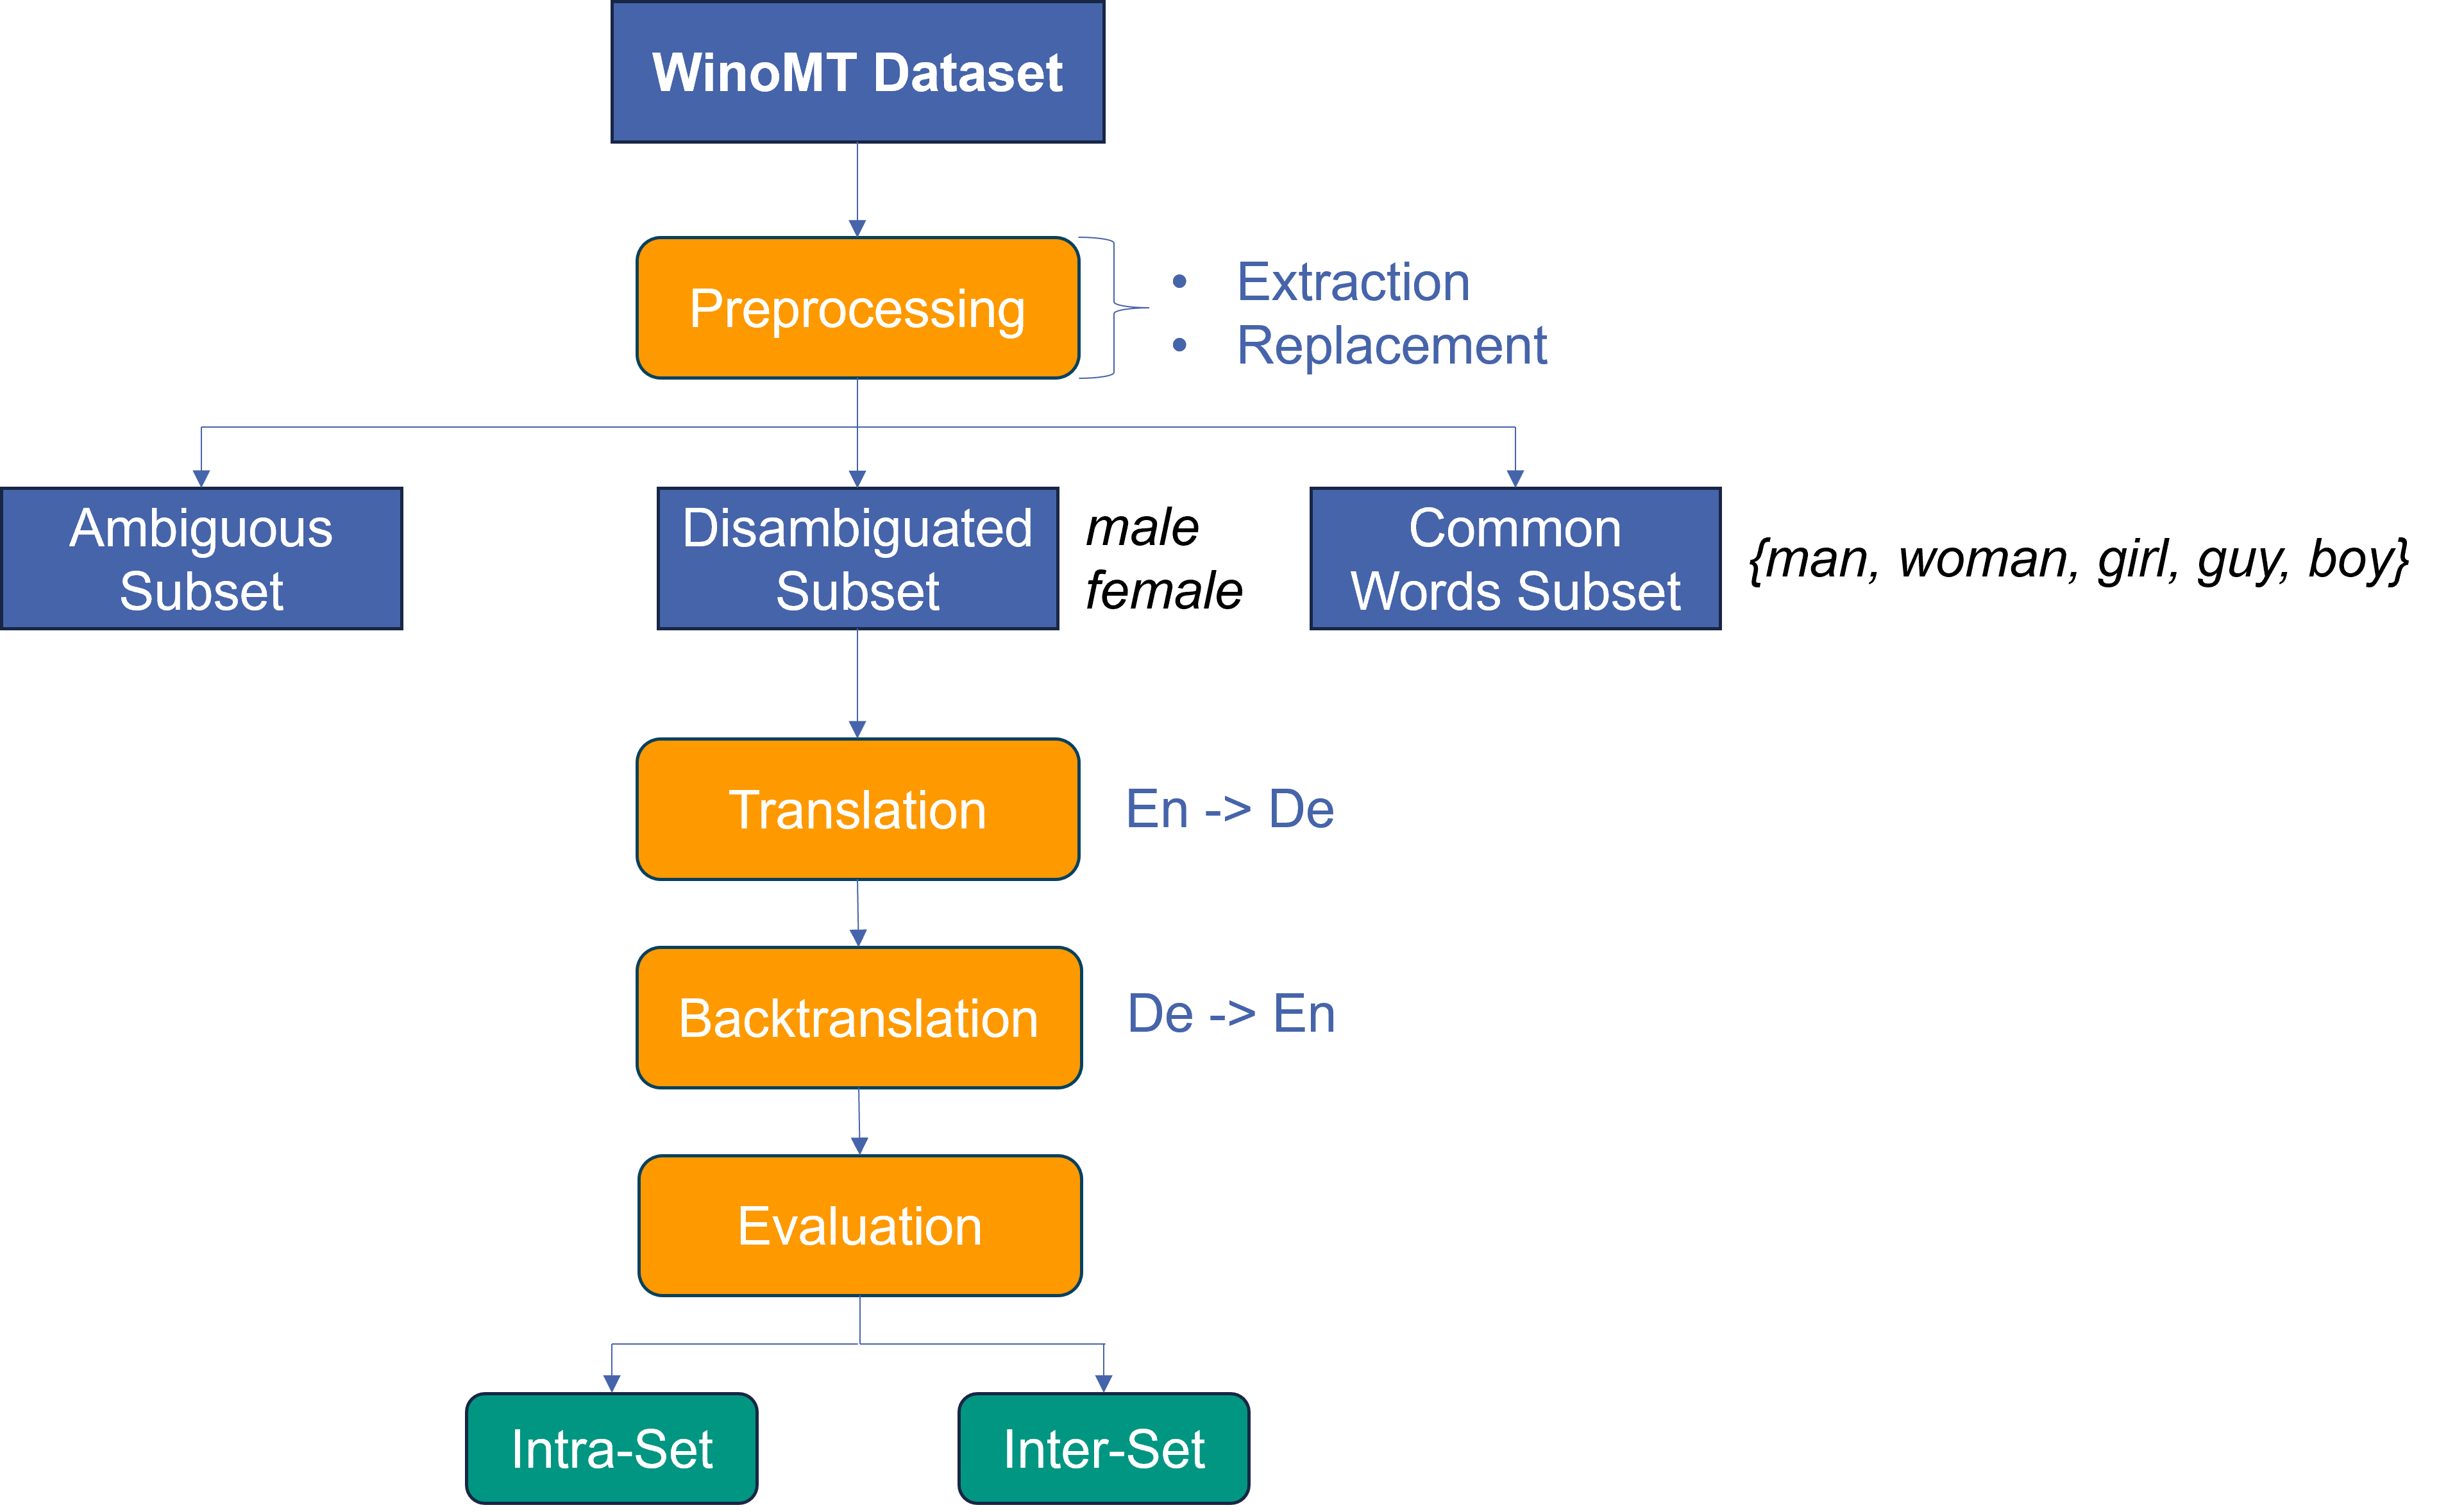
\includegraphics[scale=0.55]{figures/base_workflow.png}
  \caption{Base Experiment Workflow}
  \label{fig:base_workflow}
\end{figure}

%%%%%%%%%%%%%%%%%%%%%%%%%%%%%%%%%%%%%%%%%%%%%%%%%%%%%%%%%%%%%%%%%%%%%%%%%%%%%%%%%%%%%%%%%%%%
\section{Data Pre-processing}
\label{sec:Base_Experiment:Pre-processing}
The first step in conducting the base experiment is preprocessing the dataset. We use the artificially created WinoMT challenge set, presented in Subsection \ref{sec:Setup:Challenge_Set}. The sentences in this dataset usually consist of two gender ambiguous occupations and a context, containing disambiguation information about one of the occupations. We take the following steps to preprocess the sentences:

\begin{enumerate}
  \item \textbf{Sentence Extraction:}  
  In order to obtain fully ambiguous sentences, we remove the context information from the sentences and obtain a subset of 335 sentences from the type: "The developer argued with the designer.".
  To remove additional detection overhead, we want to have a single ambiguous word per sentence. For this purpose, we replace the second ambiguous word with a non-ambiguous proper noun, e.g. "John". 
  \item \textbf{Replacement:} 
  As next, we generate a new set of sentences, replacing the ambiguous word with different techniques:
  \begin{itemize}
      \item \textbf{Disambiguation:} We use the gender-defining adjectives \textit{male} and \textit{female} in front of the gender-ambiguous word. This technique is meant to force the translator to make the right decision regarding gender. % gender forcing
      \item \textbf{Common Words:} We replace the ambiguous word with the following common gender non-ambiguous words: \textit{man, woman, girl, guy, boy}. This method serves as a baseline for comparison against the disambiguated occupations.
  \end{itemize}
\end{enumerate}

Table \ref{tab:preprocessing} shows the generated subsets obtained by disambiguating the base ambiguous sentence "The developer argued with John.".

\begin{table}
    \begin{tabularx}{\linewidth}{|l|X|l|}
        \hline
        \textbf{Replacement Method} & \textbf{Source Sentence} & \textbf{Source Word} \\ \hline
        \multirow{2}{*}{Disambiguation} & The \textbf{male developer} argued with John. & developer \\
        & The \textbf{female developer} argued with John. & developer \\ \hline
        \multirow{5}{*}{Common Words} & The \textbf{man} argued with John. & man \\
        & The \textbf{woman} argued with John. & woman \\
        & The \textbf{girl} argued with John. & girl \\
        & The \textbf{guy} argued with John. & guy \\
        & The \textbf{boy} argued with John. & boy \\ \hline
    \end{tabularx}
    \caption{Example: Disambiguation subsets for the baseline sentence "The developer argued with John."}
    \label{tab:preprocessing}
\end{table}

%%%%%%%%%%%%%%%%%%%%%%%%%%%%%%%%%%%%%%%%%%%%%%%%%%%%%%%%%%%%%%%%%%%%%%%%%%%%%%%%%%%%%%%%%%%%
\section{Translation}
\label{sec:Base_Experiment:Translation}

The next step in conducting the experiments is translating the subsets of sentences. This is executed in two steps:

\begin{enumerate}
    \item \textbf{Translation Source -> Target:} 
    First, the subsets are translated in the target language.
    \item \textbf{Backtranslation Target -> Source:}
    The second step involves translating the translations back into the source language.
\end{enumerate}


% TODO: Decoding/search algorithm/strategy, nbest size (define what nbest means)
% We use two different decoding algorithms to compare the results: Beam search and Sampling. 
% In each step we generate nbest lists of different sizes: 10 and 100.

% ! \citet{roberts2020decoding} prove that beam search unlike sampling is skewed toward the generation of more frequent (masculine) pronouns, as it leads models to an extreme operating point that exhibits zero variability.

%%%%%%%%%%%%%%%%%%%%%%%%%%%%%%%%%%%%%%%%%%%%%%%%%%%%%%%%%%%%%%%%%%%%%%%%%%%%%%%%%%%%%%%%%%%%
\section{Word alignment}
\label{sec:Base_Experiment:Alignment}

% ??? maybe move this to Methodology, because this is the same for all experiments

In order to assign the words in the source sentence to their counterparts in the translations, we use two different alignment methods:

\begin{enumerate}
    \item Source-to-translation (\textit{fast\_align}, \textit{awesome-align}): This alignment method aligns from the source language to the target language.
    \item Translation-to-translation (\textit{Tercom}): This alignment method aligns between two translations.
\end{enumerate}

We use the first method to map each word in the source sentence to its translations and backtranslations in the target nbest lists. We do this in a two-step way, depicted in Fig. \ref{fig:alignment}. First, we align between the source sentence and the sentences in the nbest translations and extract the translations for each word. Then, we align between the translations and the backtranslations and extract the corresponding backtranslations resulting from the aligned translations of each word. 

We use the results from the second method as a baseline for comparison with the first method and to detect possible errors, which may occur in the information transfer between the two steps in the first method.

\begin{figure}
  \centering
  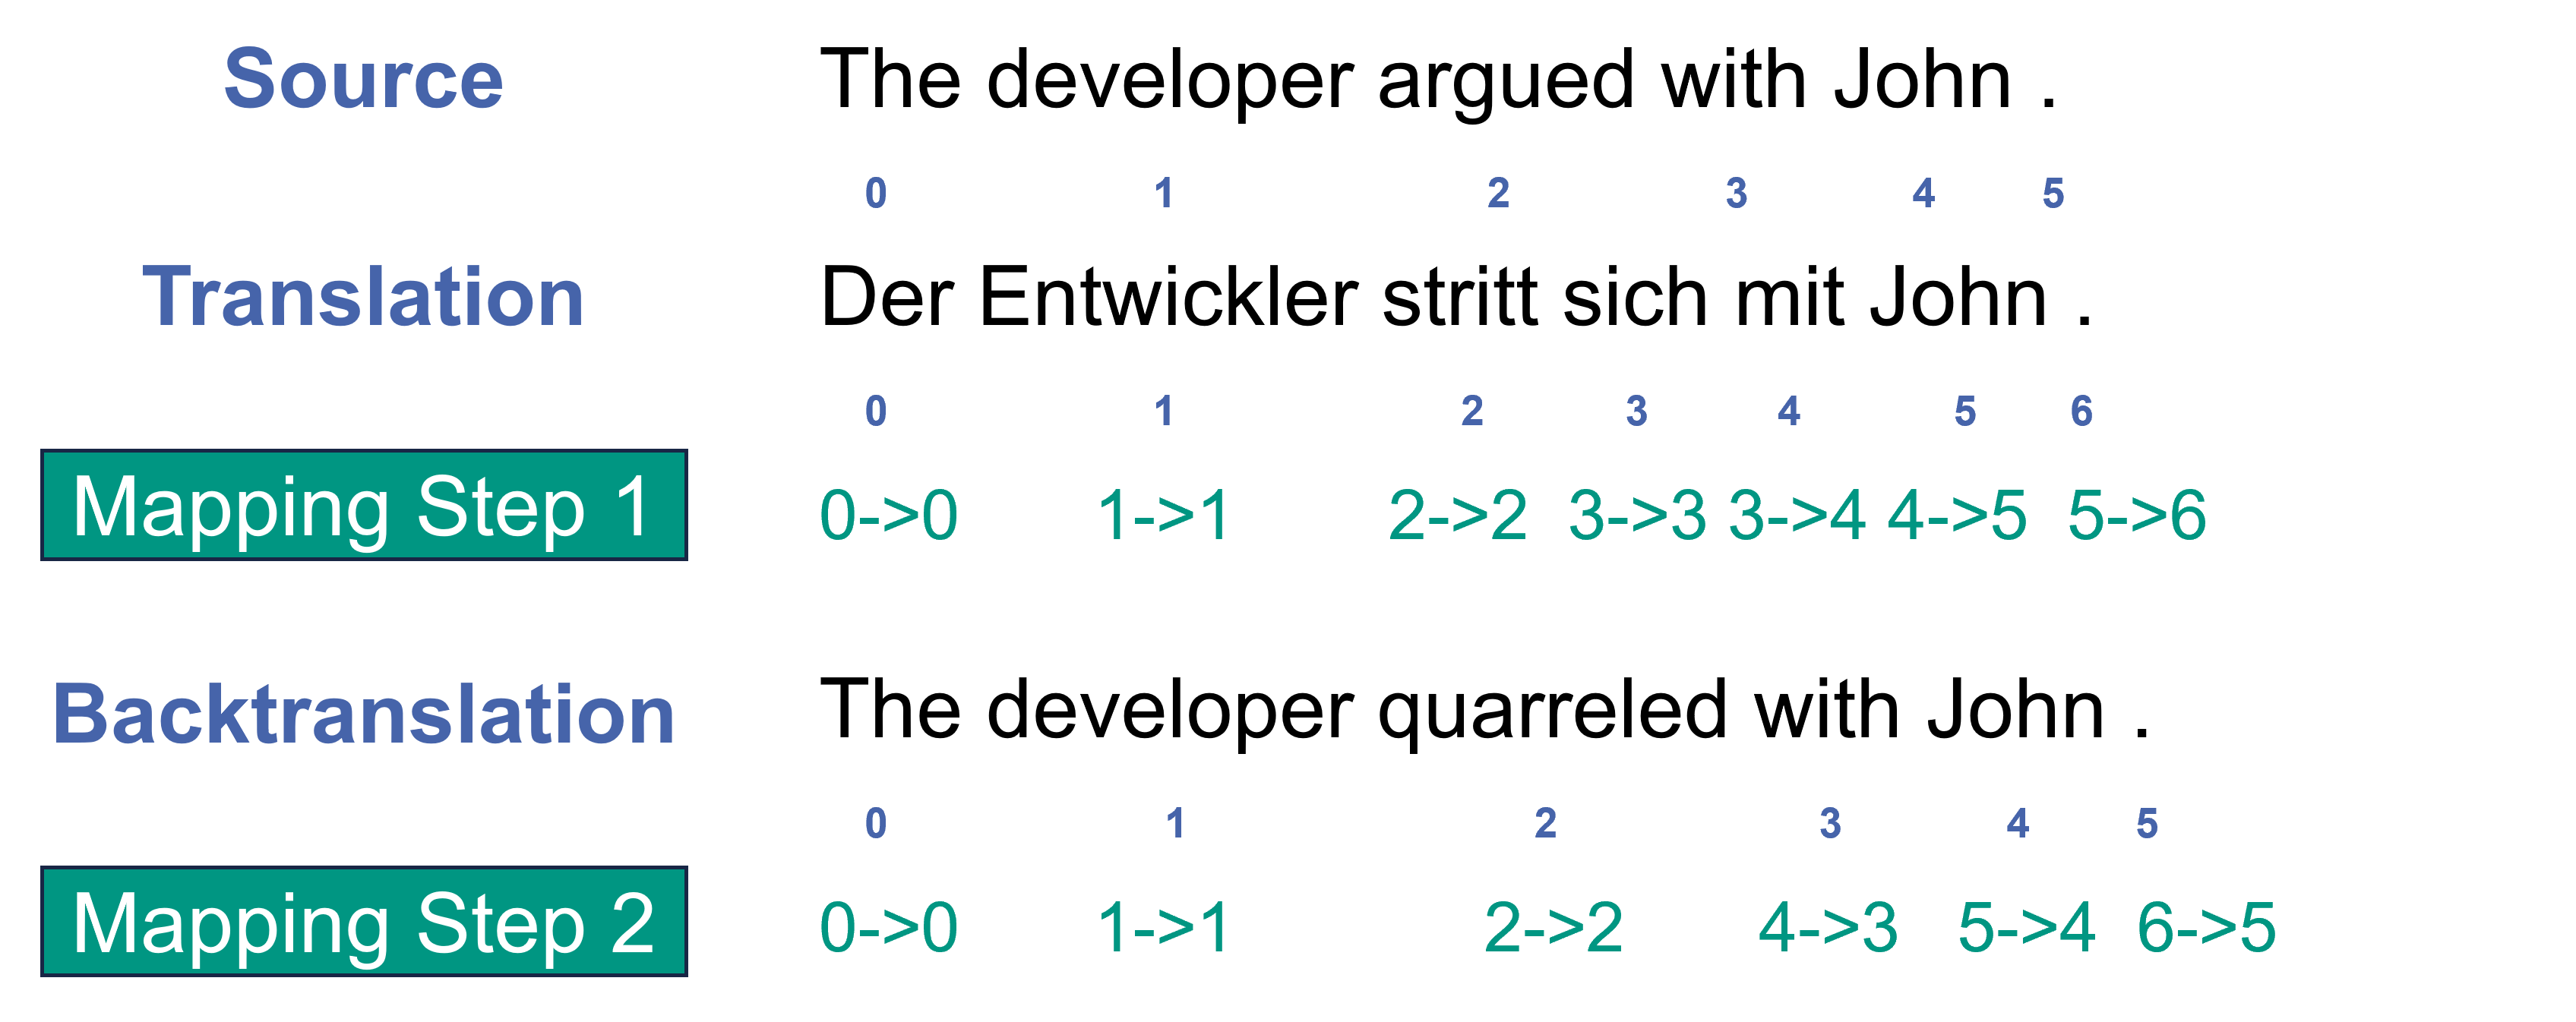
\includegraphics[scale=0.5]{figures/alignment.png}
  \caption{Example Illustration: 2-step mapping from source to translation and backtranslation}
  \label{fig:alignment}
\end{figure}

%%%%%%%%%%%%%%%%%%%%%%%%%%%%%%%%%%%%%%%%%%%%%%%%%%%%%%%%%%%%%%%%%%%%%%%%%%%%%%%%%%%%%%%%%%%%
\section{Evaluation}
\label{sec:Base_Experiment:Evaluation}

The last step in the experiments involves evaluating the translations and backtranslations to detect patterns using different statistical methods. These methods aim to probe the initial Hypothesis \ref{main}, discussed in Section \ref{sec:Methodology:Approach}. We apply all methods to all subsets and extract diversity information regarding the subsets themselves, as well as compare the results of the subsets against each other.

% TODO: define formally, maybe as a formula, pseudocode ???

%%%%%%%%%%%%%%%%%%%%%%%%%%%%%%%%%%%%%%%%%%%%%%%%%
\subsection{Recurrence Evaluation}
\label{sec:Base_Experiment:Statistics:Recurrence}
We evaluate how many of the source sentences and source words reoccur in the backtranslations:

\begin{enumerate}
    \item[1. ] Gather the backtranslations for each source sentences.
    \item[2a. ] Count the number of source sentences that reappear in their list of backtranslations.
    \item[2b. ] Count the number of source sentences which contain the source word in their list of backtranslations.
\end{enumerate}

The purpose of this evaluation is to determine which of the subsets are able to reconstruct more of the original source sentences/words.

%%%%%%%%%%%%%%%%%%%%%%%%%%%%%%%%%%%%%%%%%%%%%%%%%
\subsection{Uniqueness Evaluation}
\label{sec:Base_Experiment:Statistics:Uniqueness}
We evaluate the number of unique words and sentences in the translations and backtranslations for each sentence of the subsets. 

For the sake of the evaluation, we follow this routine (\textit{[translations | backtranslations]} denotes that we follow the same step for both the translations and backtranslations):
\begin{enumerate}
    \item[1. ] Collect the \textit{[translations | backtranslations]} for each source sentences.
    % sentence level
    \item[2a. ] Count how many of the \textit{[translations | backtranslations]} are unique. 
    % word level
    \item[2b. ] Count how many unique words there are in the \textit{[translations | backtranslations]} and normalize the number by the total amount of words. 
    \item[3. ] Average the result for all sentences.
\end{enumerate}

We use this method to probe the Hypotheses \ref{a} and \ref{b}. 

%%%%%%%%%%%%%%%%%%%%%%%%%%%%%%%%%%%%%%%%%%%%%%%%%
\subsection{Gender Evaluation}
\label{sec:Base_Experiment:Statistics:Gender}
We perform the evaluation of gender on the translations of the subsets.  First, we align each word in the source sentence with its corresponding word in the translations and backtranslations (see Subsection \ref{sec:Base_Experiment:Alignment} for more detail). Then, we perform the following steps:

\begin{enumerate}
    \item[1. ] Gather the translations of the source word for each source sentence.
    \item[2. ] Detect the gender of the translations for each source sentence.
    \item[3a. ] Determine the proportion of source sentences producing \textit{male} versus \textit{female}.
    \item[3b. ] Calculate how many of the source sentences produce \textit{both genders}. 
\end{enumerate}

The purpose of this method is to assess if the translations produce the right gender (in the non-ambiguous subsets) or both genders (in the ambiguous subset) and how often they produce both genders for each subset.

%%%%%%%%%%%%%%%%%%%%%%%%%%%%%%%%%%%%%%%%%%%%%%%%%
\subsection{Alignment Evaluation}
\label{sec:Base_Experiment:Statistics:Alignment}
Another form of evaluation is based on the alignment of the words between the source sentence, the translations and backtranslations (see Subsection \ref{sec:Base_Experiment:Alignment} for more detail).

In order to assess the translations and backtranslations of the \textbf{source word}, we do:
\begin{enumerate}
    \item[1. ] Collect all \textit{[translations | backtranslations]} of the source word.
    \item[2. ] Count how many of the \textit{[translations | backtranslations]} are unique.
    \item[3. ] Average the result for all sentences.
\end{enumerate}

Similarly, to assess the translations and backtranslations of the \textbf{rest of the sentence} excluding the source word, we do:
\begin{enumerate}
    \item[1. ] Collect all \textit{[translations | backtranslations]} of the sentence rest.
    \item[2. ] Count how many of the \textit{[translations | backtranslations]} are unique.
    \item[3. ] Average the result for all sentences.
\end{enumerate}

The idea behind this evaluation method is to assess the Hypothesis \ref{c}.

Next, we will present the results of these statistical evaluations of the subsets.

%%%%%%%%%%%%%%%%%%%%%%%%%%%%%%%%%%%%%%%%%%%%%%%%%%%%%%%%%%%%%%%%%%%%%%%%%%%%%%%%%%%%%%%%%%%%
\section{Results}
\label{ch:Base_Experiment:Results}

% - Translation quality
% - Gender bias quality

% Finding patterns in statistical results
% e.g. influence of language, context

% BLEU score on WinoMT: not possible, because no reference translations

% Variables to consider:
% - Word alignment method
% - Disambiguation method 
% ?- Search method
% - Nbest size


%%%%%%%%%%%%%%%%%%%%%%%%%%%%%%%%%%%%%%%%%%%%%%%%%
\subsection{Recurrence Evaluation Results}
\label{ch:Base_Experiment:Results:Recurrence}

The results from the evaluation of recurrence for beam search with beam size 10 are listed in Table \ref{tab:recurrence_10}.
% Highest score
As we can observe, the average from the subsets of common words presents the highest score in both the recurring sentences and words. This is to be expected, because the words in these subsets are most generic and have the highest probability of being predicted, compared to the occupational words from the WinoMT sentences in the other three subsets. 

% Interesting findings
Most interestingly, the female-disambiaguated subset has the lowest score for occurring sentences. When investigating the results, we found some discrepancy between the way "female" and "male" are translated. The "female" prefix is very often lost in the backtranslation, which results in the backtranslated sentence being regarded as differing from the source sentence. In contrast, the "male" prefix is most often preserved, resulting in the same sentence in backtranslation. We illustrate this with the following examples:

\begin{itemize}
    \item \textbf{Source (EN):} The \textit{female} developer argued with John. \\
    \textbf{Translation (DE):} Die Entwicklerin argumentierte mit John. \\
    \textbf{Backtranslation (EN):} The developer argued with John.
    
    \item \textbf{Source (EN):} The \textit{male} developer argued with John. \\
    \textbf{Translation (DE):} Der \textit{männliche} Entwickler argumentierte mit John. \\
    \textbf{Backtranslation (EN):} The \textit{male} developer argued with John.
\end{itemize}

As we can see, the "male" prefix is translated to its corresponding word in German "männliche", while the "female" prefix is lost in the translation, but its meaning is reflected in the female gender of the German word for developer "Entwicklerin".

Also, both disambiguation subsets sometimes generate the opposite gender with the correct prefix, for example, "der \textit{weibliche} Entwickler" (the \textit{female} male developer) and "die \textit{männliche} Entwicklerin" (the \textit{male} female developer). This presents a contradiction that influences the . 

We note that the findings from these results are important and will have an effect on the further experiments.

Table \ref{tab:recurrence_100} shows the results from the evaluation of recurrence for beam search with beam size 100. Here we can observe that more female sentences are reoccurring in backtranslation compared to beam 100, which means that increasing the beam increases the possibility for preservation of the "female" prefix.
Also, with beam size 100 the source word reappears for all source sentences in the backtranslations.

\begin{table} 
    \begin{tabularx}{\linewidth}{|X|XXXX|}
        \hline
         & \textbf{Ambiguous} & \textbf{Disambiguated (male)} & \textbf{Disambiguated (female)} & \textbf{Non-ambiguous average} \\ \hline
         \textbf{Sentences} & 295/335 & 293/335 & 118/335 & \underline{308/335} \\ 
         \textbf{Words} & 329/335 & 330/335 & 314/335 & \underline{335/335} \\ \hline
    \end{tabularx}
    \caption{\textbf{Recurrence Evaluation Results: Beam Size 10}. English-German. Backtranslation. Beam search with beam size 10. Nbest size 10. Highest scores are underlined. \\ First row: number of source sentences that reappear in the backtranslations. \\ Second row: number of source sentences which contain the source word in the backtranslations.}
    \label{tab:recurrence_10}
\end{table}

\begin{table} 
    \begin{tabularx}{\linewidth}{|X|XXXX|}
        \hline
         & \textbf{Ambiguous} & \textbf{Disambiguated (male)} & \textbf{Disambiguated (female)} & \textbf{Non-ambiguous average} \\ \hline
         \textbf{Sentences} & 329/335 & \underline{330/335} & 281/335 & 329/335 \\ 
         \textbf{Words} & 335/335 & 335/335 & 335/335 & 335/335 \\ \hline
    \end{tabularx}
    \caption{\textbf{Recurrence Evaluation Results: Beam Size 100}. English-German. Backtranslation. Beam search with beam size 100. Nbest size 100. Highest scores are underlined. \\ First row: number of source sentences that reappear in the backtranslations. \\ Second row: number of source sentences which contain the source word in the backtranslations.}
    \label{tab:recurrence_100}
\end{table}

%%%%%%%%%%%%%%%%%%%%%%%%%%%%%%%%%%%%%%%%%%%%%%%%%
\subsection{Uniqueness Evaluation Results}
\label{ch:Base_Experiment:Results:Uniqueness}

The results from the evaluation of uniqueness are listed in Table \ref{tab:uniqueness_translation} for translation and Table \ref{tab:uniqueness_backtranslation} for backtranslation.
Since we use the beam search algorithm for decoding with beam size 10 and nbest size 10, we expect it to generate 10 unique sentences per translation, which is almost always the case, as we see from the score for the number of unique sentences in translations. 

% Interesting findings
Most notable are the results for the number of unique backtranslations. As we can see, the ambiguous subset produces the least amount of unique sentences in backtranslation, which proves Hyp. \ref{a}. In Table \ref{tab:uniqueness_backtranslation_100} we can see the results for number of unique backtranslations with beam size 100, which confirm this result. However, when regarding the results for the different common words separately instead of averaged, as we can see in Fig. \ref{fig:range}, the minimum value in the range, 43.9 (for the word "boy") for beam size 10 and 3074.01 (for the word "guy") for beam size 100, is still lower for the common words compared to the ambiguous subset, 45.98 for beam size 10 and 3181.51 for beam size 100.

The results for the number of unique words in translation and backtranslation are inconclusive. Considering Hyp. \ref{b}, we expected the ambiguous subset to generate the least unique words in backtranslation, but this is not the case.

\begin{table} 
    \begin{tabularx}{\linewidth}{|X|XXXX|}
        \hline
         & \textbf{Ambiguous} & \textbf{Disambiguated (male)} & \textbf{Disambiguated (female)} & \textbf{Non-ambiguous average} \\ \hline
         \textbf{Sentences} & 9.94/10 & 9.95/10 & 9.87/10 & \underline{9.97/10} \\ 
         \textbf{Words} & \underline{0.205} & 0.19 & 0.201 & 0.202 \\ \hline
    \end{tabularx}
    \caption{\textbf{Uniqueness Evaluation Results for Translation}. English-German. Beam search with beam size 10. Nbest size 10. Highest scores are underlined. \\ First row: Averaged number of unique sentences per source sentence out of 10 translations. \\ Second row: Averaged number of unique words per source sentence, normalized by the average total number of words in 10 translations.}
    \label{tab:uniqueness_translation}
\end{table}

\begin{table} 
    \begin{tabularx}{\linewidth}{|X|XXXX|}
        \hline
         & \textbf{Ambiguous} & \textbf{Disambiguated (male)} & \textbf{Disambiguated (female)} & \textbf{Non-ambiguous average} \\ \hline
         \textbf{Sentences} & 45.98/100 & 50.73/100 & \underline{50.82/100} & 47.06/100 \\ 
         \textbf{Words} & 0.044 & 0.039 & 0.043 & \underline{0.045} \\ \hline
    \end{tabularx}
    \caption{\textbf{Uniqueness Evaluation Results for Backtranslation: Beam Size 10}. English-German. Beam search with beam size 10. Nbest size 10. Best results are underlined. \\ First row: Averaged number of unique sentences per source sentence out of 10 translations. \\ Second row: Averaged number of unique words per source sentence, normalized by the average total number of words in 100 backtranslations.}    \label{tab:uniqueness_backtranslation}
\end{table}

\begin{table} 
    \begin{tabularx}{\linewidth}{|X|XXXX|}
        \hline
         & \textbf{Ambiguous} & \textbf{Disambiguated (male)} & \textbf{Disambiguated (female)} & \textbf{Non-ambiguous average} \\ \hline
         \textbf{Sentences} & 3181.51/10000 & 3391.55/10000 & \underline{3424.98/10000} & 3297.48/10000 \\ \hline
    \end{tabularx}
    \caption{\textbf{Uniqueness Evaluation Results for Backtranslation: Beam Size 100}. English-German. Beam search with beam size 100. Nbest size 100. Best results are underlined. \\ First row: Averaged number of unique sentences per source sentence out of 100 translations. \\ Second row: Averaged number of unique words per source sentence, normalized by the average total number of words in 10000 backtranslations.}
    \label{tab:uniqueness_backtranslation_100}
\end{table}

%%% Range of uniqueness
\begin{figure}
     \centering
     
     \begin{subfigure}{0.49\textwidth}
         \centering
         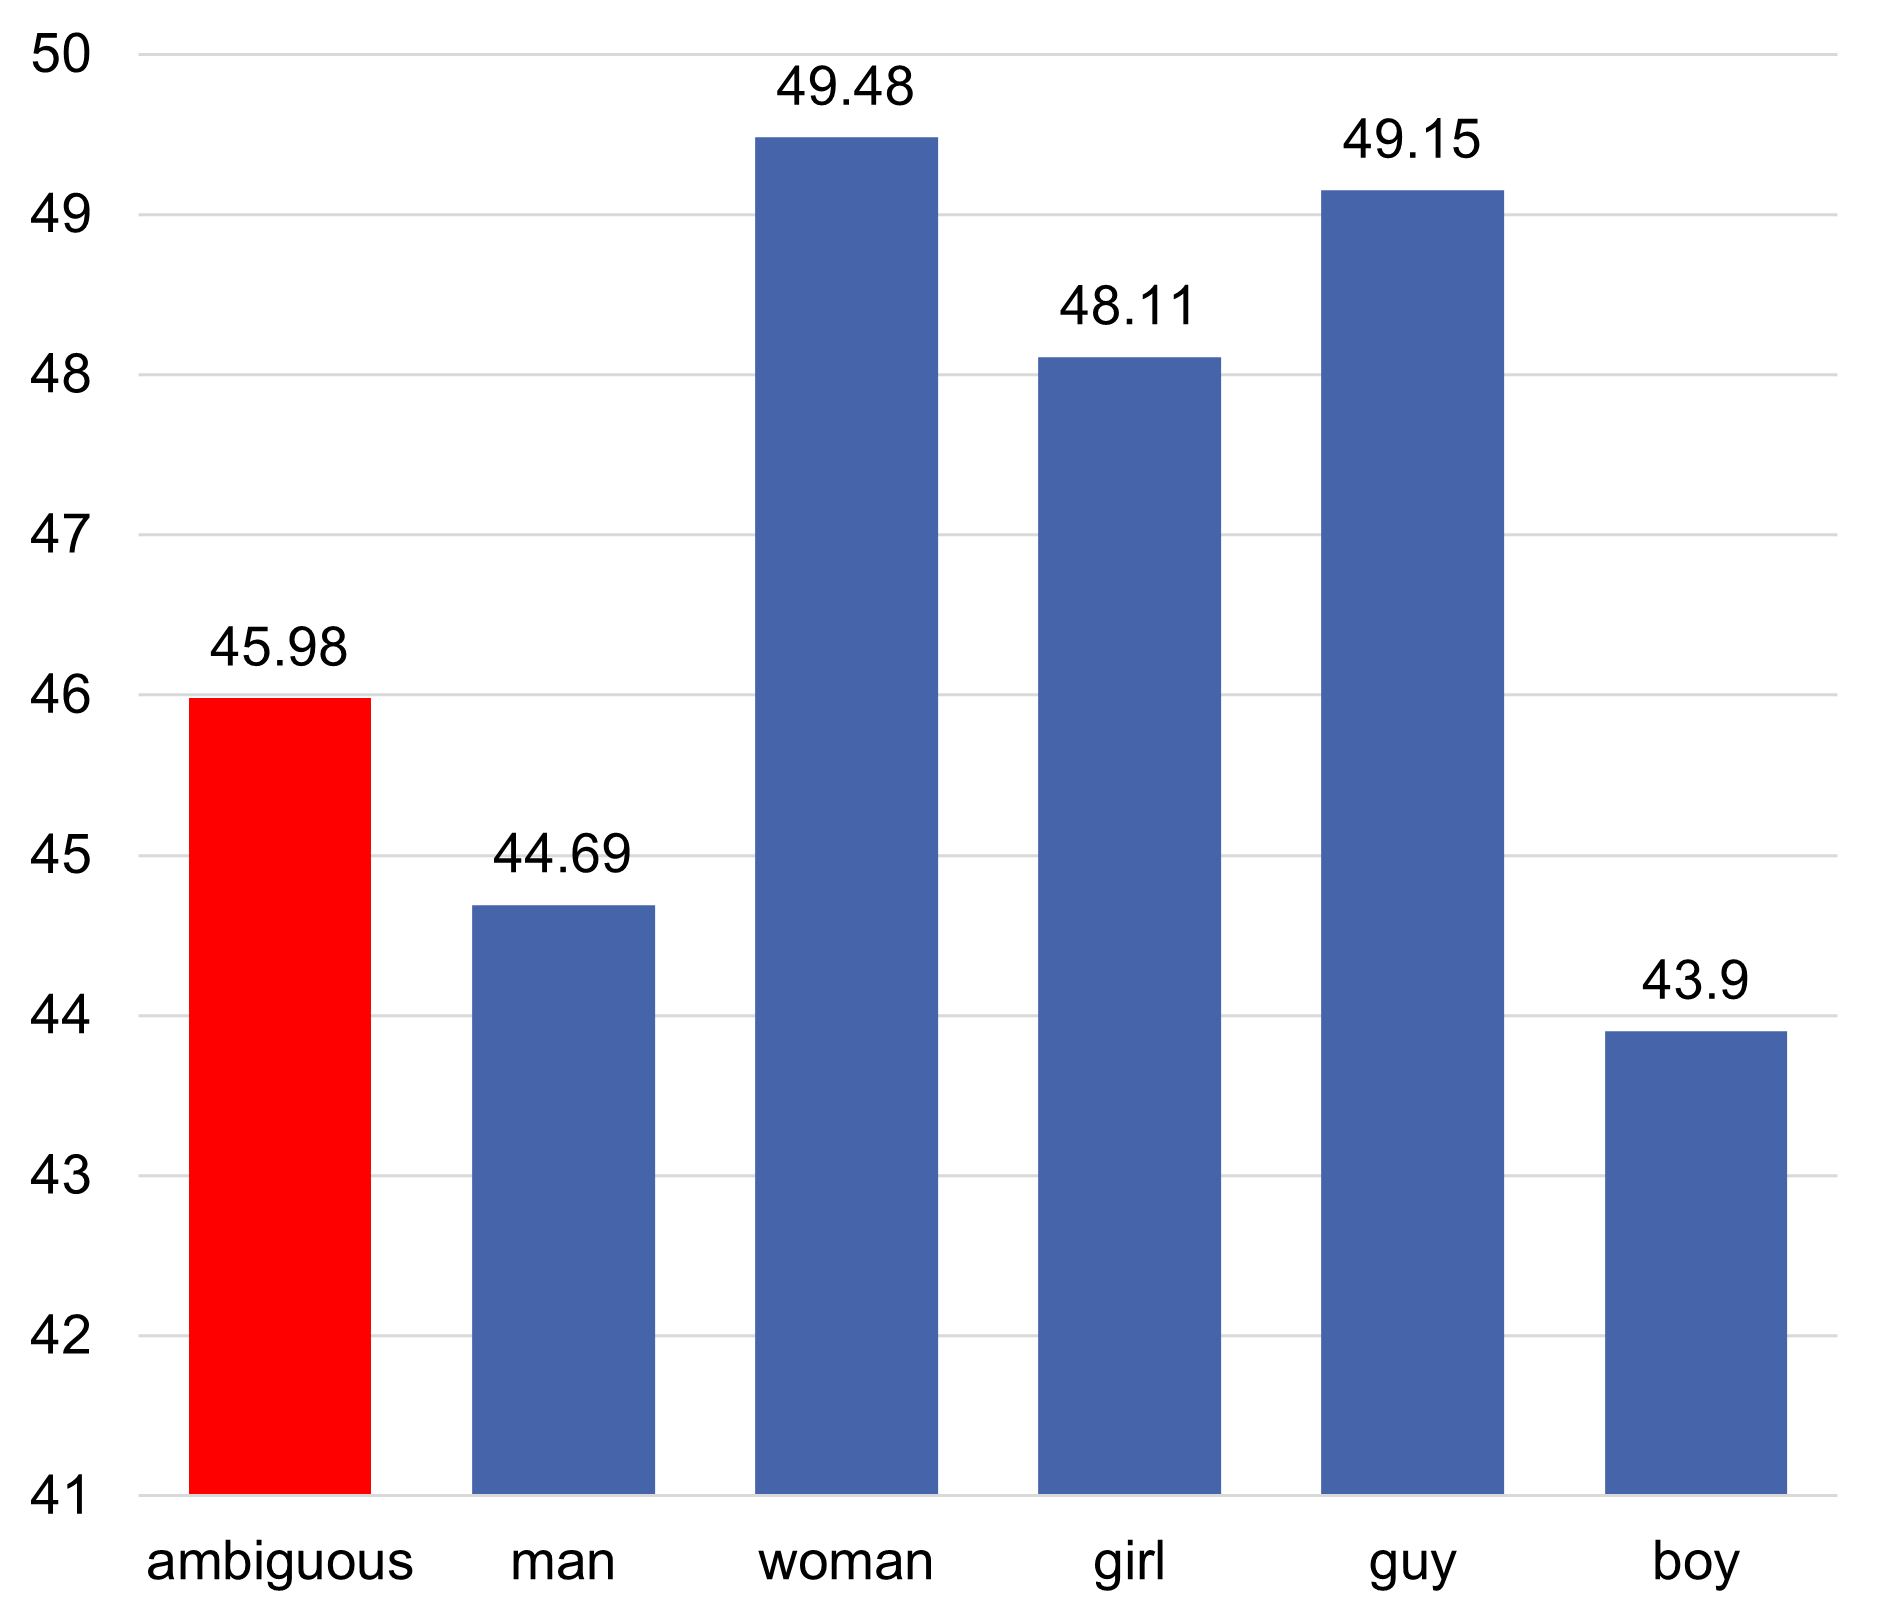
\includegraphics[width=\textwidth]{figures/uniqueness/range_beam_10.png}
         \caption{Beam 10}
         \label{fig:three sin x}
     \end{subfigure}
     \hfill
     \begin{subfigure}{0.49\textwidth}
         \centering
         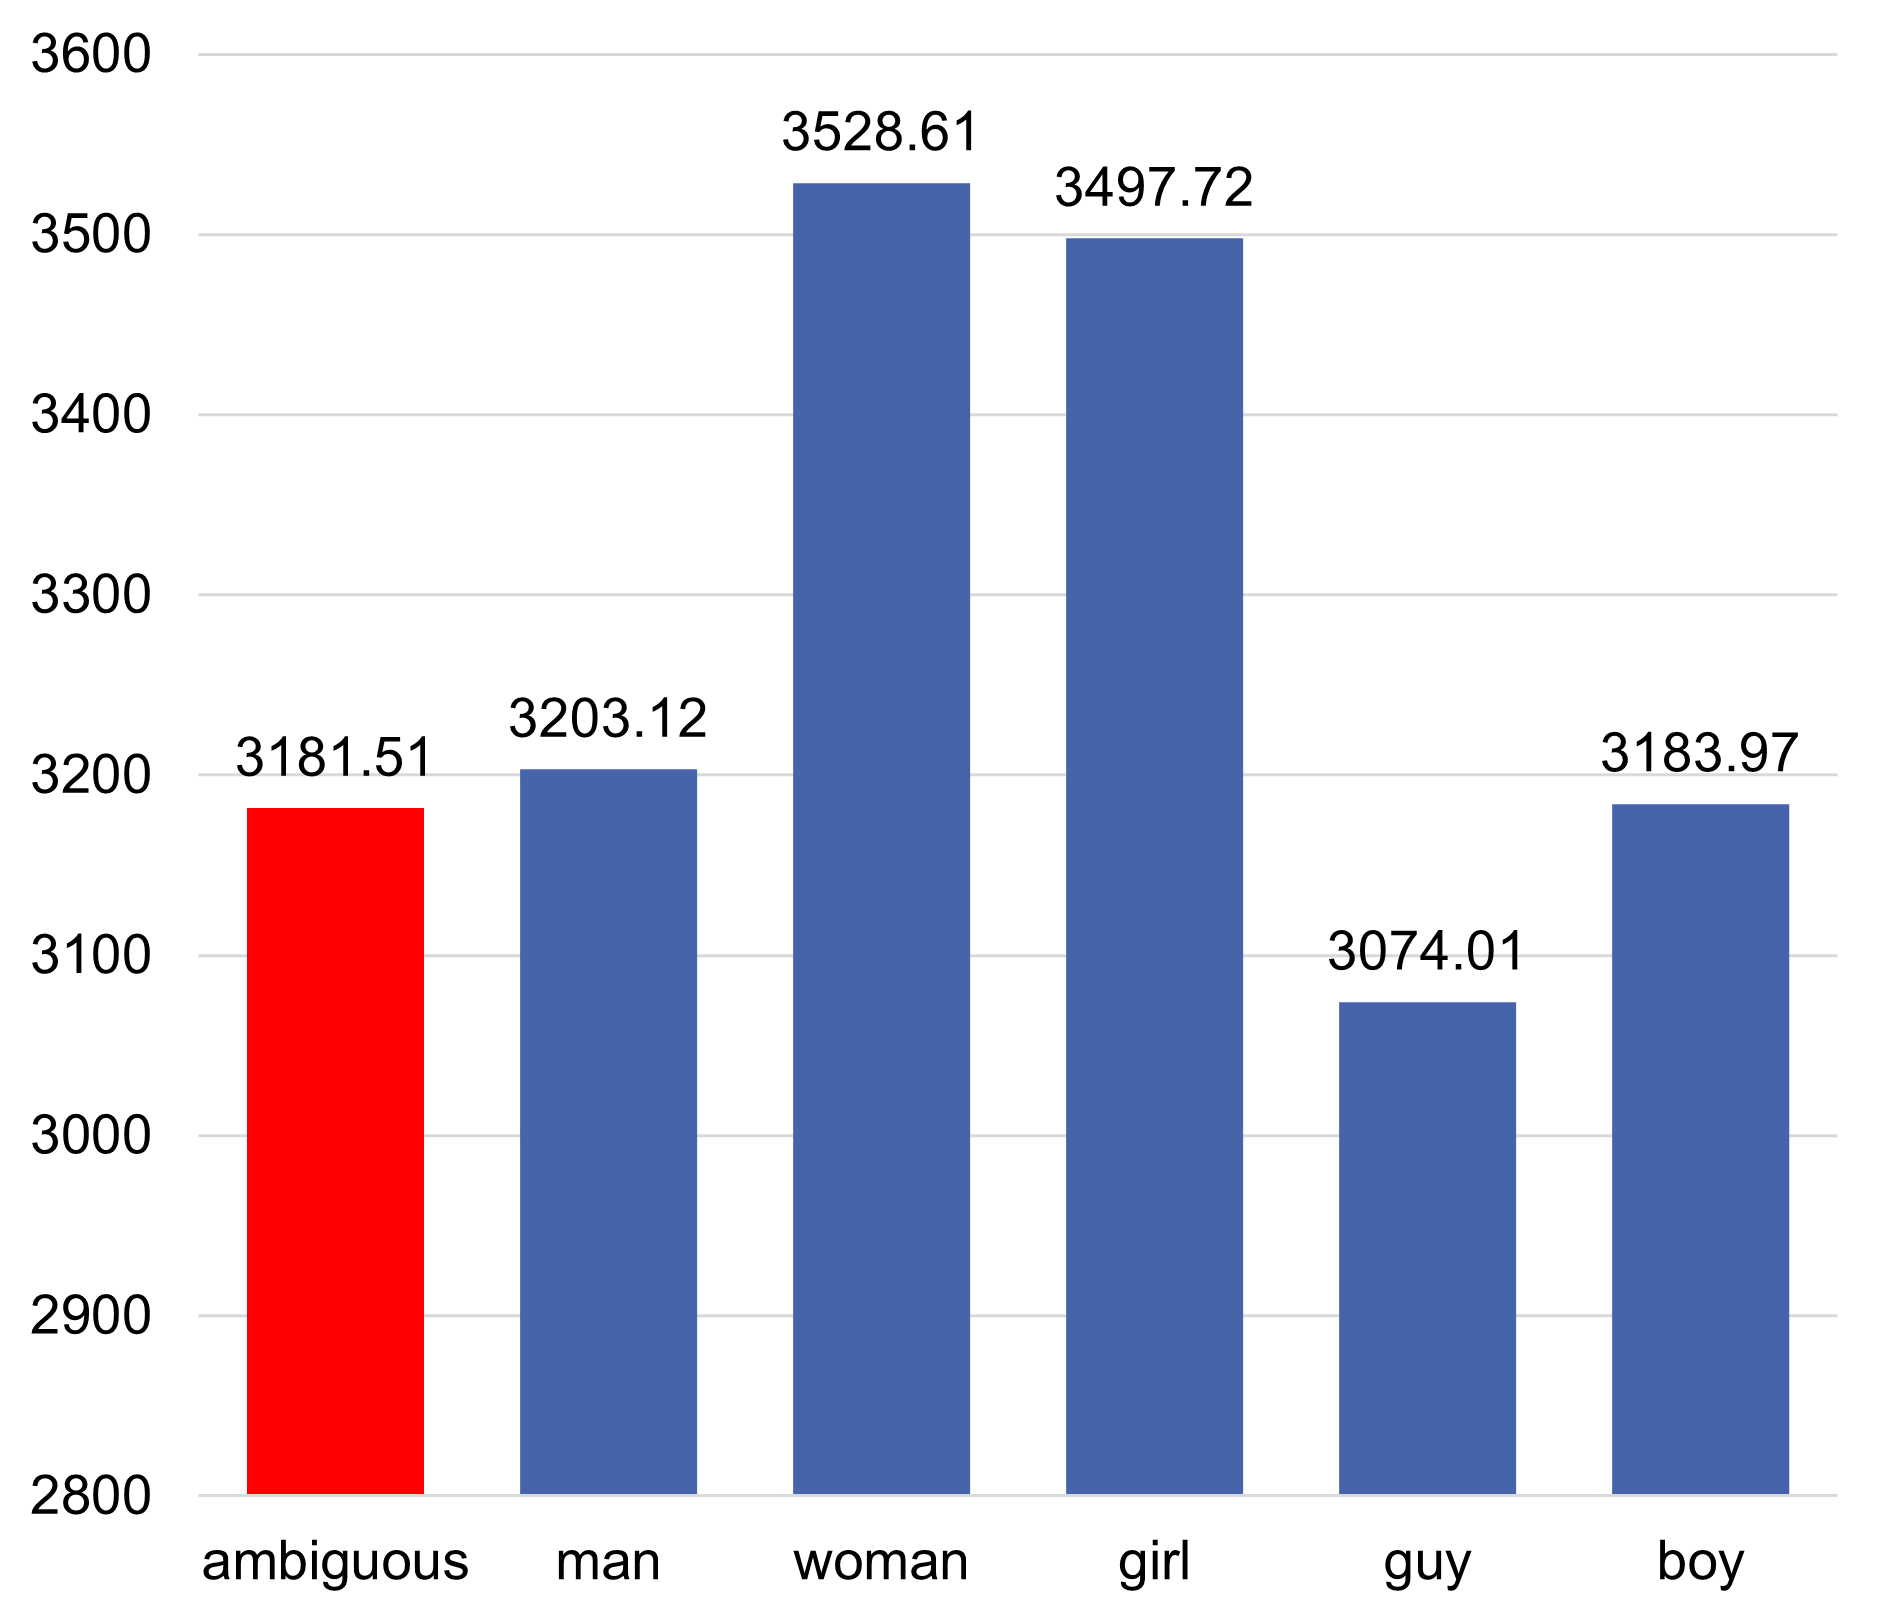
\includegraphics[width=\textwidth]{figures/uniqueness/range_beam_100.png}
         \caption{Beam 100}
         \label{fig:five over x}
     \end{subfigure}
     
    \caption{Comparison Between the Number of Unique Backtranslations for Common Words and Ambiguous Subsets}
    \label{fig:range}

\end{figure}

%%%%%%%%%%%%%%%%%%%%%%%%%%%%%%%%%%%%%%%%%%%%%%%%%
\subsection{Gender Evaluation Results}
\label{ch:Base_Experiment:Results:Gender}

The results from the evaluation of gender are listed in Table \ref{tab:gender_percent_10} for beam size 10 and in Table \ref{tab:gender_percent_100} for beam size 100. We can observe that, as expected, the subset of disambiguated with "male" sentences has predominantly male translations, and similarly the subset of disambiguated with "female" sentences has mostly female translations. The same applies to the male words "man", "guy" and "boy", as well as the female word "woman". The female word "girl" presents an exception, because in German it is a neutral noun.

Also, as expected, the ambiguous source sentences produce the most translations of both genders, while the common non-ambiguous words produce the least. Despite this, the disambiguation subsets still have a rather high amount of sentences producing both genders. 

Interestingly, when comparing the disambiguation subsets, the disambiguation with "female" seems to be more successful overall, with more sentences producing the right gender and less of both genders appearing in the translations.

Fig. \ref{fig:gender_pie_10} further shows the influence of increasing the beam size tenfold. We can observe that more of both genders occur in translation with beam 100 compared to beam 10. Also, there is more balance between female and male in the translations of the ambiguous subset, with the difference between 78.66\% and 14.88\% being smaller than between 86.27\% and 12.81\%. But on the other hand, more male gender translations occur in the female-disambiguated subset, which is a downside.

\begin{table} 
    \begin{tabularx}{\linewidth}{|X|XXXX|}
        \hline
         & \textbf{Ambiguous} & \textbf{Disambiguated (male)} & \textbf{Disambiguated (female)} & \textbf{Non-ambiguous} \\ \hline
         \textbf{Male} & 86.27\% & 89.46\% & 6.81\% & \textit{man}: 95.01\% \\
         &&&& \textit{woman}: 0.51\% \\
         &&&& \textit{girl}: 0.39\% \\
         &&&& \textit{guy}: 93.07\% \\
         &&&& \textit{boy}: \underline{96.15\%} \\ \hline
         \textbf{Female} & 12.81\% & 11.19\% & 92.33\% & \textit{man}: 0.18\% \\ 
         &&&& \textit{woman}: \underline{96.69\%} \\
         &&&& \textit{girl}: 0.81\% \\
         &&&& \textit{guy}: 0.18\% \\
         &&&& \textit{boy}: 0.27\% \\\hline
         \textbf{Both genders} & \underline{38.21\%} & 35.22\% & 28.06\% & average: 0.72\% \\ \hline
    \end{tabularx}
    \caption{\textbf{Gender Evaluation Results: Beam Size 10}. English-German. Translation. Beam search with beam size 10. Nbest size 10. Highest scores are underlined. \\ First and second row: Percentage of the source sentences producing male versus female translations. \\ Third row: Percentage of the source sentences producing both genders in translation.}
    \label{tab:gender_percent_10}
\end{table}

\begin{table} 
    \begin{tabularx}{\linewidth}{|X|XXXX|}
        \hline
         & \textbf{Ambiguous} & \textbf{Disambiguated (male)} & \textbf{Disambiguated (female)} & \textbf{Non-ambiguous} \\ \hline
         \textbf{Male} & 78.66\% & 81.96\% & 8.27\% & \textit{man}: 83.80\% \\
         &&&& \textit{woman}: 0.59\% \\
         &&&& \textit{girl}: 0.75\% \\
         &&&& \textit{guy}: 78.59\% \\
         &&&& \textit{boy}: \underline{86.48\%} \\ \hline
         \textbf{Female} & 14.88\% & 14.24\% & 86.90\% & \textit{man}: 0.46\% \\ 
         &&&& \textit{woman}: \underline{88.57\%} \\
         &&&& \textit{girl}: 5.66\% \\
         &&&& \textit{guy}: 0.98\% \\
         &&&& \textit{boy}: 0.75\% \\\hline
         \textbf{Both genders} & \underline{91.64\%} & 91.34\% & 82.98\% & average: 23.04\% \\ \hline
    \end{tabularx}
    \caption{\textbf{Gender Evaluation Results: Beam Size 100}. English-German. Translation. Beam search with beam size 100. Nbest size 100. Highest scores are underlined. \\ First and second row: Percentage of the source sentences producing male versus female translations. \\ Third row: Percentage of the source sentences producing both genders in translation.}
    \label{tab:gender_percent_100}
\end{table}

%%% Pie charts
\begin{figure}
     \centering
     
     \begin{subfigure}{\textwidth}
         \centering
         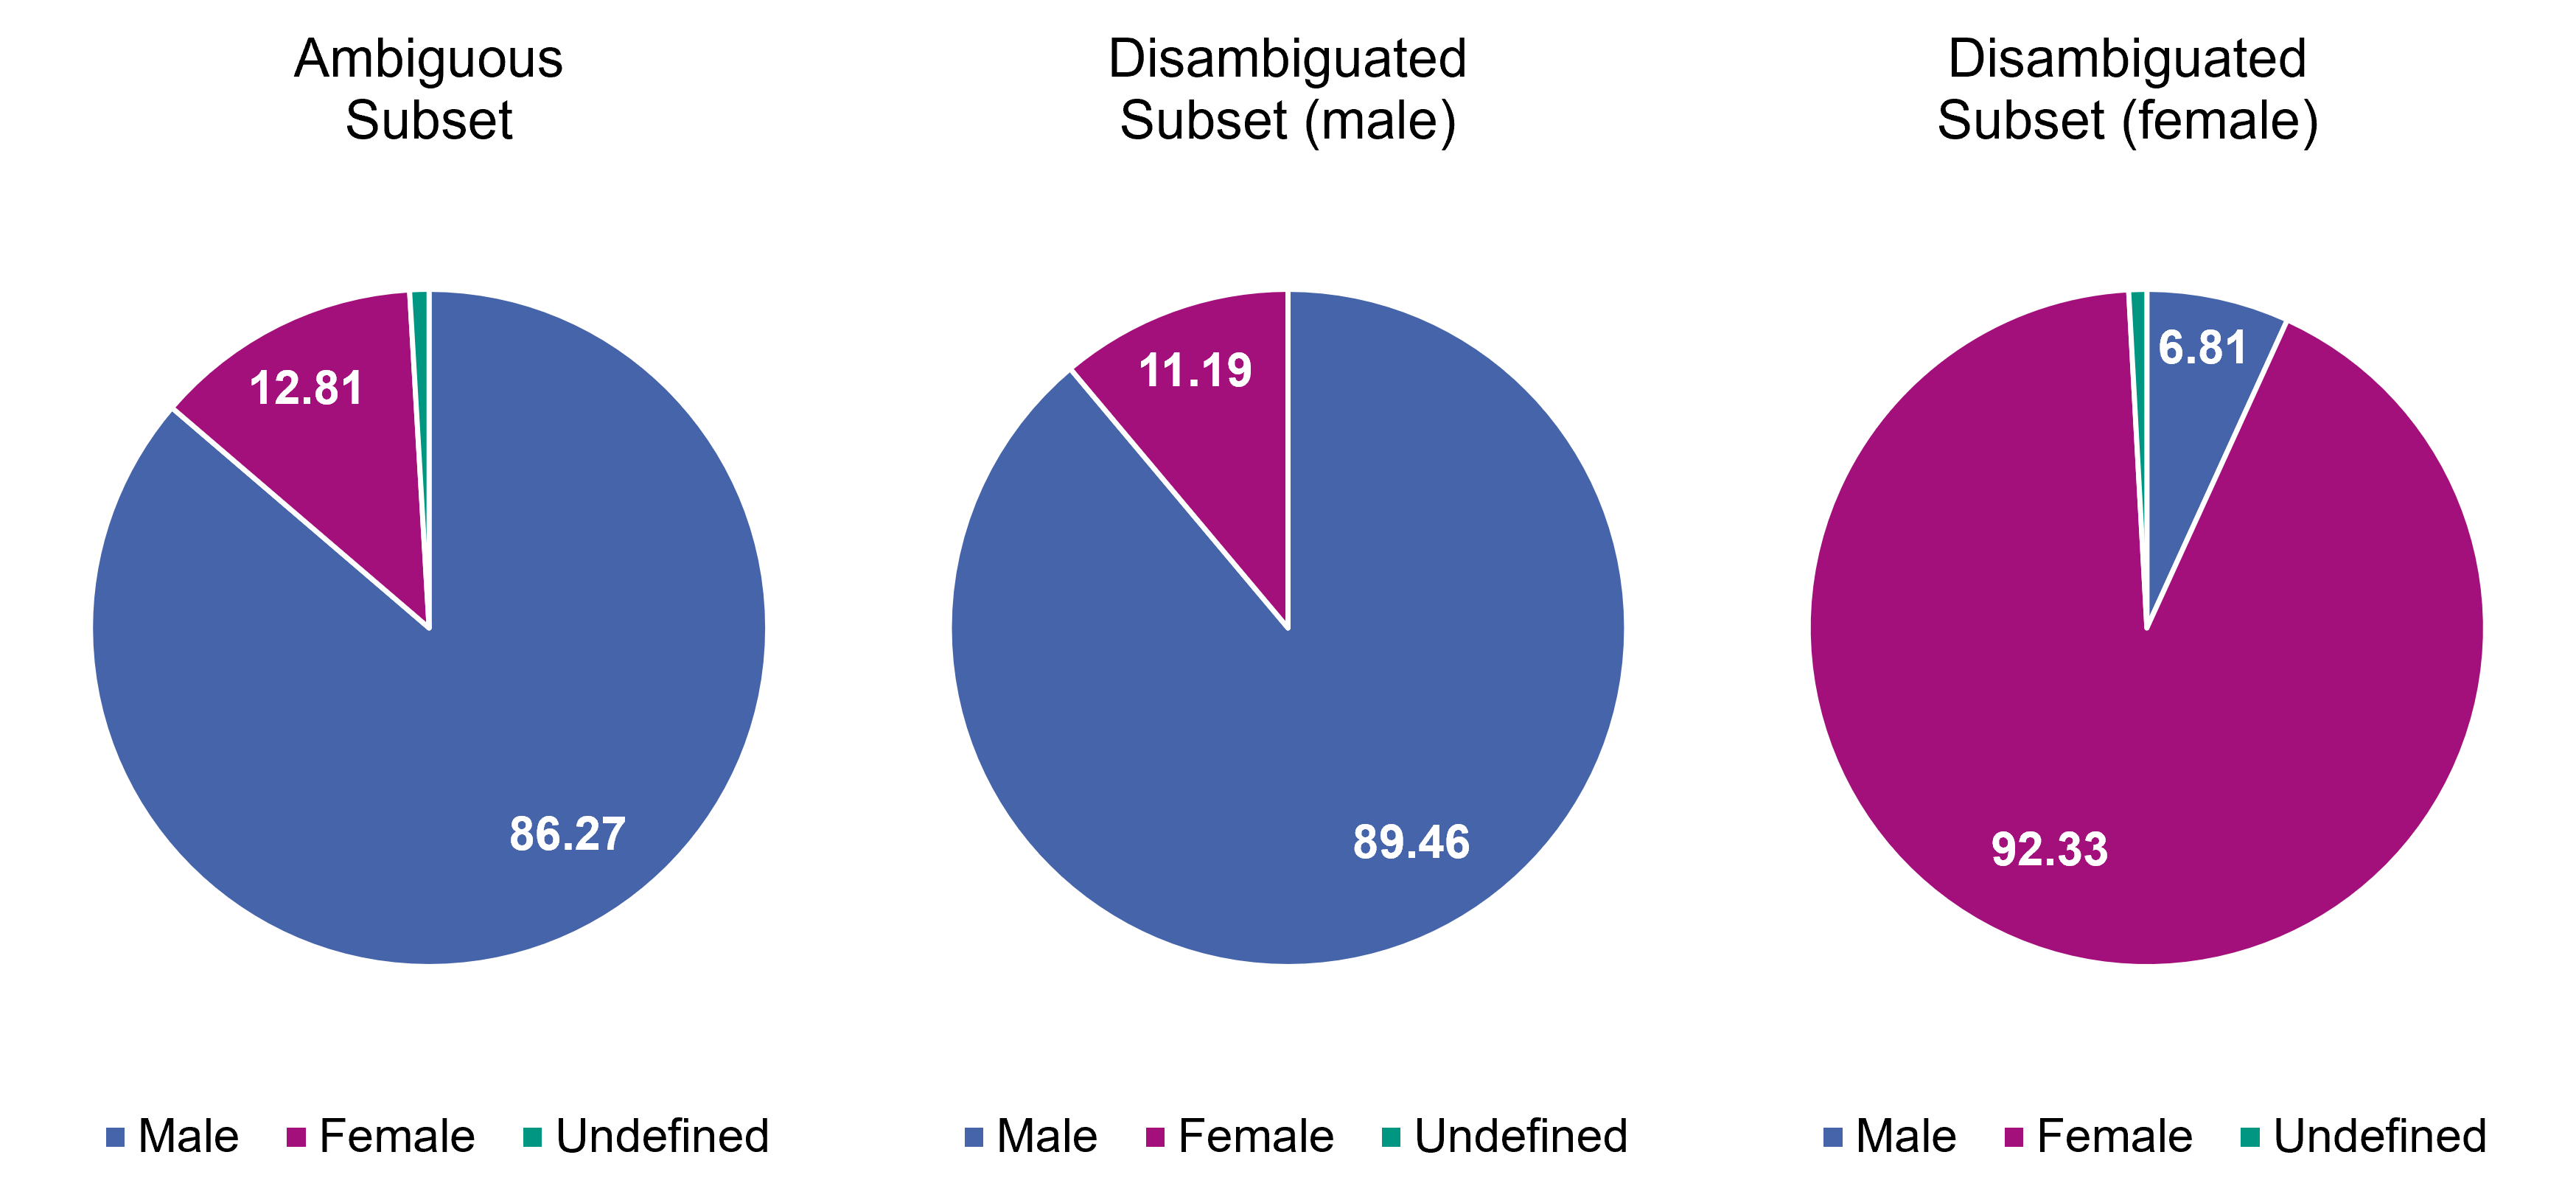
\includegraphics[width=\textwidth]{figures/gender/beam_10.png}
         \caption{Beam 10}
         \label{fig:three sin x}
     \end{subfigure}
     
     \begin{subfigure}{\textwidth}
         \centering
         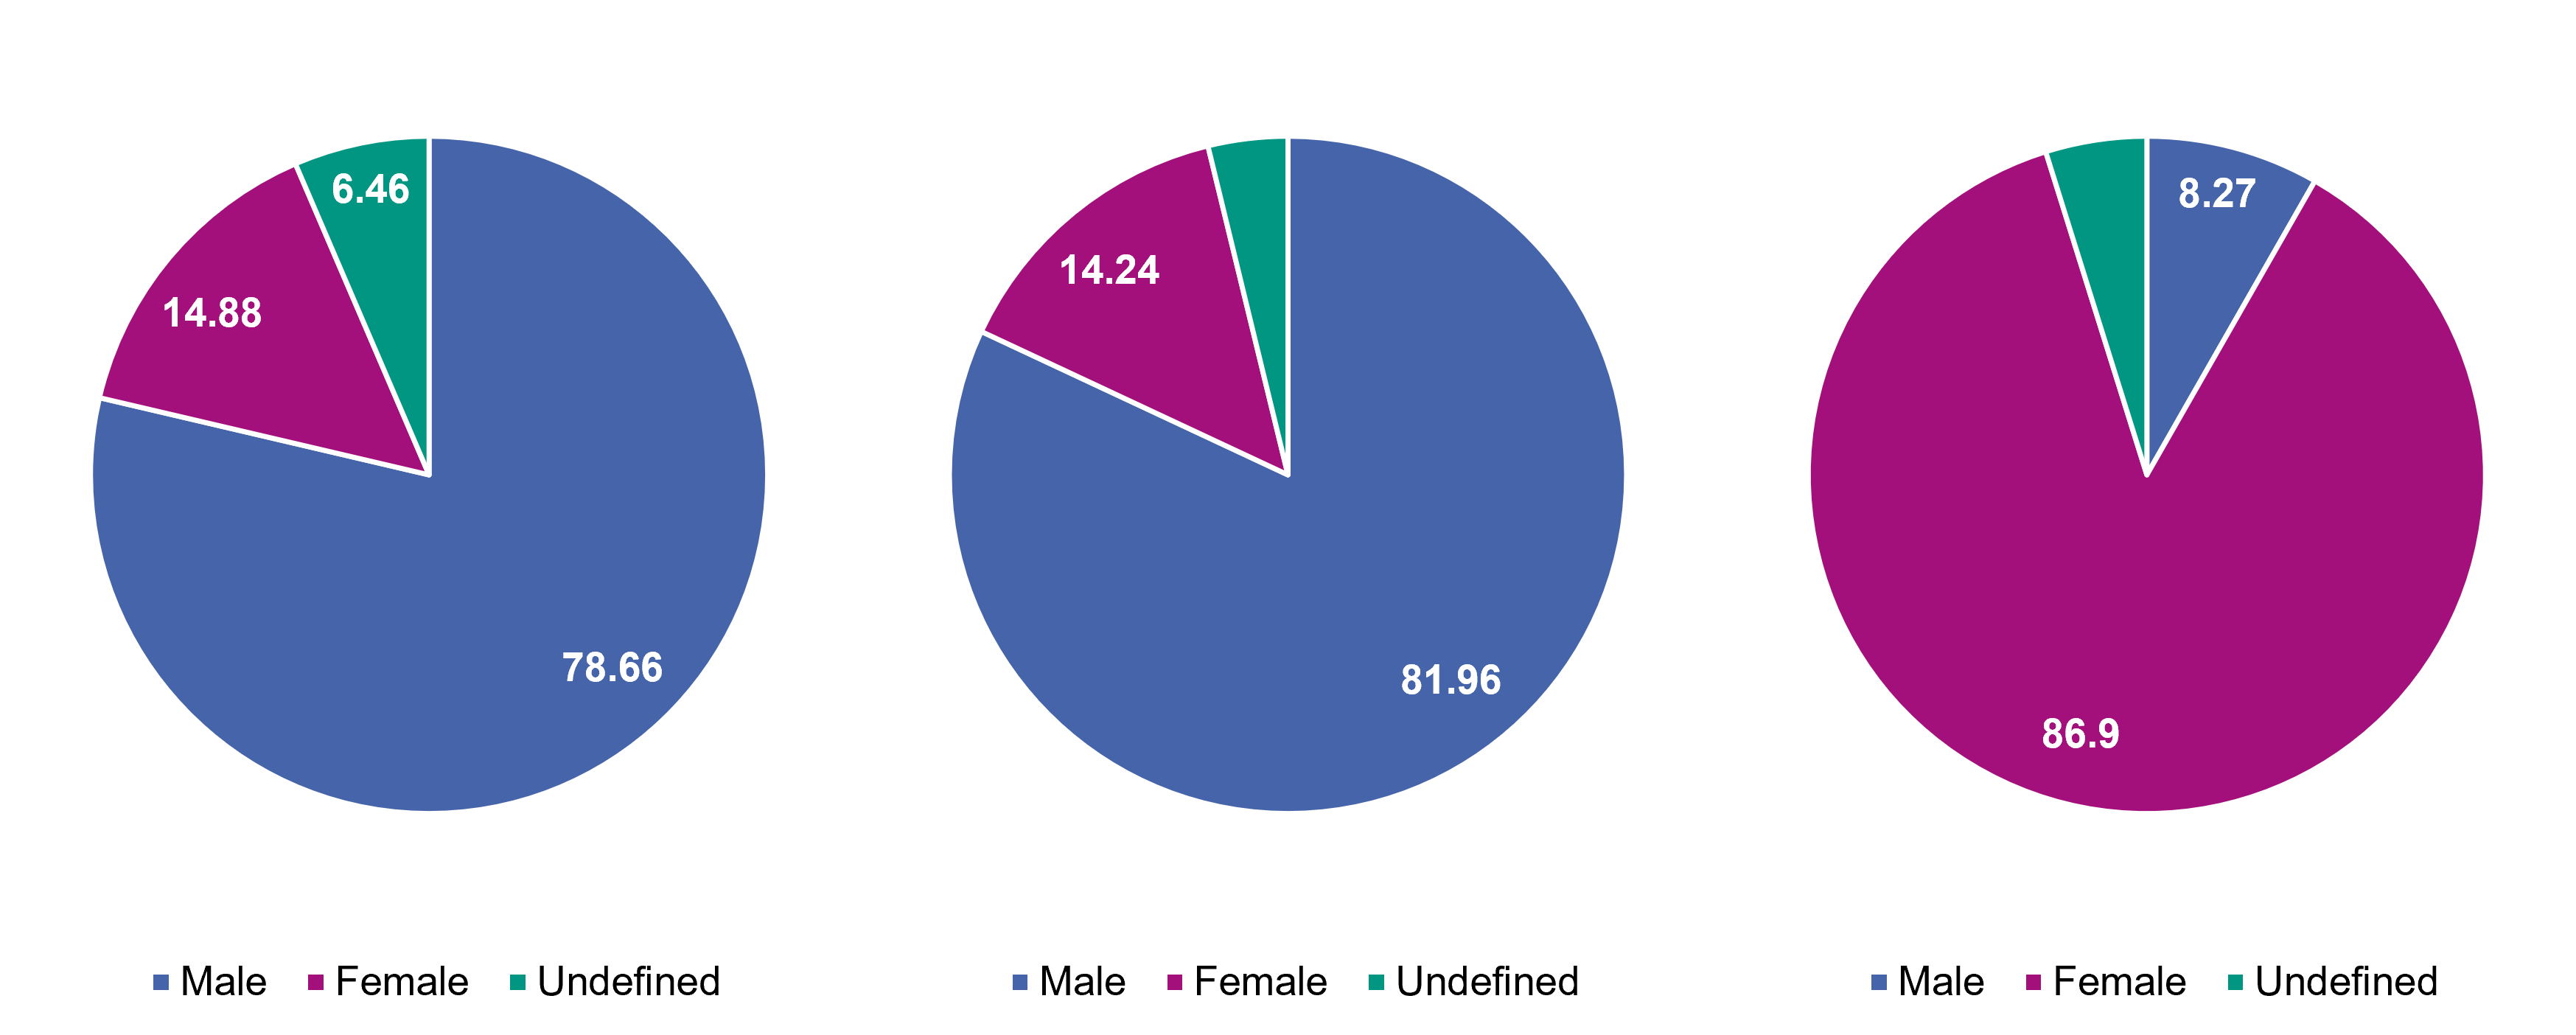
\includegraphics[width=\textwidth]{figures/gender/beam_100.png}
         \caption{Beam 100}
         \label{fig:five over x}
     \end{subfigure}
     
     
    \caption{Gender Representation in Translation}
    \label{fig:gender_pie_10}
\end{figure}

%%%%%%%%%%%%%%%%%%%%%%%%%%%%%%%%%%%%%%%%%%%%%%%%%
\subsection{Alignment Evaluation Results}
\label{ch:Base_Experiment:Results:Alignment}

The results from the evaluation of gender for beam 10 and 100 are listed in Tables \ref{tab:alignment_translation_10} and \ref{tab:alignment_translation_100} for translation and Tables \ref{tab:alignment_backtranslation_10} and \ref{tab:alignment_backtranslation_100} for backtranslation.

% ??? - The rest of the sentence excluding the ambiguous word should have more unique words than the rest of the sentence excluding the disambigauted word
% ??? - The ambiguous word in a sentence generates more unique words in backtranslation than the rest of the sentence.

% Translation
The alignment results for translation feature unique words with and without gender information. For example, the male and female German word for developer: "Entwickler" and "Entwicklerin", are considered one unique word when disregarding gender information. The removal of gender information is performed using a rule-based approach. Despite this, the assumption that this would reduce the number of unique words for the ambiguous subset compared to the other subsets, is not entirely confirmed. This is only the case when we compare the female-disambiguated subset with the ambiguous subset.


% Difference between unique words per ambiguous words vs. rest of sentence for original and unambiguous words average (2.38 – 1.87 vs 1.70 – 1.94)
A notable trend in the results is that the non-ambiguous subset has the significantly lowest score in uniqueness for the translations of the source word, but it also has the highest score for the rest of the sentence. But also, the scores for the source word and the rest of the sentence are closer together for the non-ambiguous subset than the scores for the ambiguous subset. This is also an indication of the stronger tendency of the decoding algorithm to put more emphasis on the ambiguous word rather than the rest of the sentence, when such an ambiguous word is present.

The results for beam size 100 also show a similar trend.

% Backtranslation
While the results from the translation are not conclusive, the results from the backtranslation exhibit a noticeable pattern. We can see that for the source word, the non-ambiguous subset has the least amount of unique backtranslations, contrary to the expectation from Hyp. \ref{c}, which postulated that the ambiguous subset should produce the least unique backtranslations. However, the ambiguous subset has less unique translations than the female-disambiguated subset, which partially confirms the hypothesis. The same results are observed with beam size 100.

% Interesting results
Interestingly, for beam size 10, both in translation and backtranslation the rest of the sentence for the non-ambiguous subset produces the most diverse translations compared to the ambiguous subset. This may indicate that more emphasis is given on diversity of the rest of the sentence, when the source word is unambiguous itself. However, the same observation cannot be made for beam size 100, where the rest of the sentence for the ambiguous subset produces the most diverse translations.

% TODO: Difference between FA and AA

\begin{table} 
    \begin{tabularx}{\linewidth}{|X|XXXX|}
        \hline
         & \textbf{Ambiguous} & \textbf{Disambiguated (male)} & \textbf{Disambiguated (female)} & \textbf{Non-ambiguous average} \\ \hline
         \textbf{Source word (FA, WIG)} & 2.87/10 & 2.83/10 & \underline{3.02/10} & 1.83/10 \\
         \textbf{Source word (FA, WOG)} & 2.66/10 & 2.64/10 & \underline{2.81/10} & 1.83/10 \\
         \textbf{Source word (AA, WIG)} & 2.38/10 & \underline{2.43/10} & 2.33/10 & 1.70/10 \\ 
         \textbf{Source word (AA, WOG)} & 2.66/10 & 2.64/10 & \underline{2.81/10} & 1.83/10 \\\hline 
         \textbf{Sentence rest (AA)} & 1.87/10 & 1.67/10 & 1.64/10 & \underline{1.94/10} \\ \hline
    \end{tabularx}
    \caption{\textbf{Alignment Evaluation Results for Translation: Beam Size 10}. English-German. Beam search with beam size 10. Nbest size 10. Highest scores are underlined. FA: \textit{fast\_align}, AA: \textit{awesome-align}. WIG (with gender): gender information preserved, WOG (without gender): gender information removed. \\ First and second row: Averaged number of unique translations of the source word per source sentence in the 10 translations. \\ Third row: Averaged number of unique translations of the sentence rest per source sentence in the 10 translations.}
    \label{tab:alignment_translation_10}
\end{table}

\begin{table} 
    \begin{tabularx}{\linewidth}{|X|XXXX|}
        \hline
         & \textbf{Ambiguous} & \textbf{Disambiguated (male)} & \textbf{Disambiguated (female)} & \textbf{Non-ambiguous average} \\ \hline
         \textbf{Source word (FA, WIG)} & 12.37/100 & 13.70/100 & \underline{14.76/100} & 7.18/100 \\
         \textbf{Source word (FA, WOG)} & 11.04/100 & 12.47/100 & \underline{13.38/100} & 7.18/100 \\
         \textbf{Source word (AA, WIG)} & 10.81/100 & 12.12/100 & \underline{13.12/100} & 5.26/100 \\ 
         \textbf{Source word (AA, WOG)} & 9.46/100 & 10.88/100 & \underline{11.75/100} & 5.26/100 \\\hline 
         \textbf{Sentence rest (AA)} & 6.52/100 & 5.39/100 & 5.85/100 & \underline{7.23/100} \\ \hline
    \end{tabularx}
    \caption{\textbf{Alignment Evaluation Results for Translation: Beam Size 100}. English-German. Beam search with beam size 100. Nbest size 100. Highest scores are underlined. FA: \textit{fast\_align}, AA: \textit{awesome-align}. WIG (with gender): gender information preserved, WOG (without gender): gender information removed. \\ First and second row: Averaged number of unique translations of the source word per source sentence in the 100 translations. \\ Third row: Averaged number of unique translations of the sentence rest per source sentence in the 100 translations.}
    \label{tab:alignment_translation_100}
\end{table}

\begin{table} 
    \begin{tabularx}{\linewidth}{|X|XXXX|}
        \hline
         & \textbf{Ambiguous} & \textbf{Disambiguated (male)} & \textbf{Disambiguated (female)} & \textbf{Non-ambiguous average} \\ \hline
         \textbf{Source word (FA)} & 8.84/100 & 8.32/100 & \underline{9.79/100} & 5.25/100 \\ 
         \textbf{Source word (AA)} & 7.48/100 & 7.04/100 & \underline{7.85/100} & 4.80/100 \\ 
         \textbf{Source word (Tercom)} & 8.02/100 & 7.90/100 & \underline{9.82/100} & 6.52/100 \\ \hline
         \textbf{Sentence rest (AA)} & 4.13/100 & 3.72/100 & 3.73/100 & \underline{4.66/100} \\ \hline
    \end{tabularx}
    \caption{\textbf{Alignment Evaluation Results for Backtranslation}. English-German. Beam search with beam size 10. Nbest size 10. Highest scores are underlined. FA: \textit{fast\_align}, AA: \textit{awesome-align}. \\ First-third row: Averaged number of unique backtranslations of the source word per source sentence in the 100 backtranslations. \\ Fourth row: Averaged number of unique backtranslations of the sentence rest per source sentence in the 100 backtranslations.}
    \label{tab:alignment_backtranslation_10}
\end{table}

\begin{table} 
    \begin{tabularx}{\linewidth}{|X|XXXX|}
        \hline
         & \textbf{Ambiguous} & \textbf{Disambiguated (male)} & \textbf{Disambiguated (female)} & \textbf{Non-ambiguous average} \\ \hline
         \textbf{Source word (FA)} & 147.93/10000 & 148.34/10000 & \underline{163.53/10000} & 69.76/10000 \\ 
         \textbf{Source word (AA)} & 120.08/10000 & 121.96/10000 & \underline{136.14/10000} & 48.82/10000 \\ \hline 
         \textbf{Sentence rest (AA)} & \underline{68.00/10000} & 66.39/10000 & 63.41/10000 & 66.06/10000 \\ \hline
    \end{tabularx}
    \caption{\textbf{Alignment Evaluation Results for Backtranslation}. English-German. Beam search with beam size 100. Nbest size 100. Highest scores are underlined. FA: \textit{fast\_align}, AA: \textit{awesome-align}. \\ First-third row: Averaged number of unique backtranslations of the source word per source sentence in the 10000 backtranslations. \\ Fourth row: Averaged number of unique backtranslations of the sentence rest per source sentence in the 10000 backtranslations.}
    \label{tab:alignment_backtranslation_100}
\end{table}




% Test

Test fig. \ref{fig:three graphs}

\begin{figure}
     \centering
     
     \begin{subfigure}{0.49\textwidth}
         \centering
         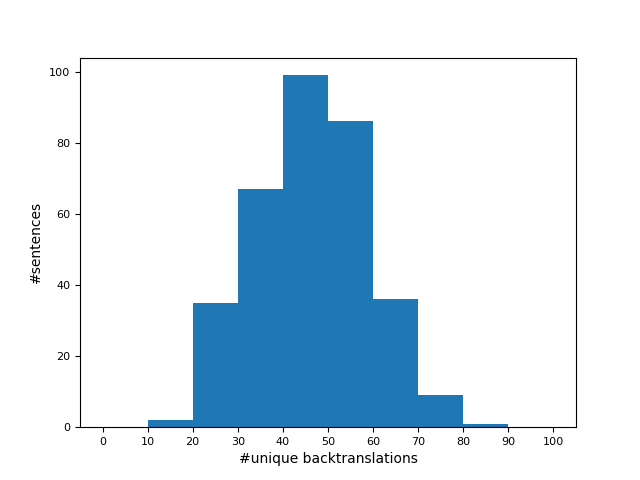
\includegraphics[width=\textwidth]{figures/unique_back_original.png}
         \caption{$y=3\sin x$}
         \label{fig:three sin x}
     \end{subfigure}
     \hfill
     \begin{subfigure}{0.49\textwidth}
         \centering
         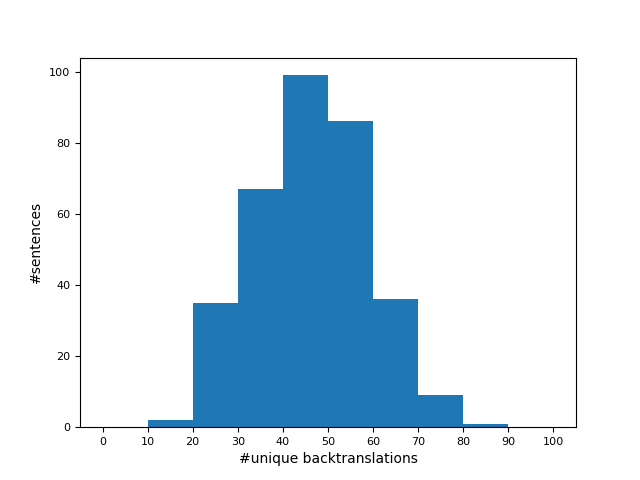
\includegraphics[width=\textwidth]{figures/unique_back_original.png}
         \caption{$y=5/x$}
         \label{fig:five over x}
     \end{subfigure}
     \begin{subfigure}{0.49\textwidth}
         \centering
         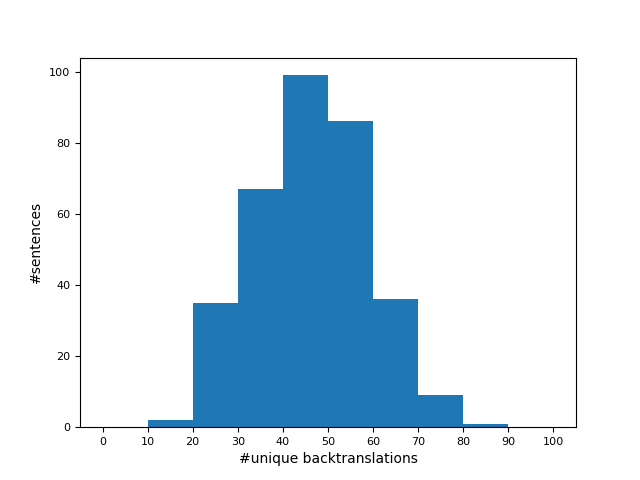
\includegraphics[width=\textwidth]{figures/unique_back_original.png}
         \caption{$y=3\sin x$}
         \label{fig:three sin x}
     \end{subfigure}
     \hfill
     \begin{subfigure}{0.49\textwidth}
         \centering
         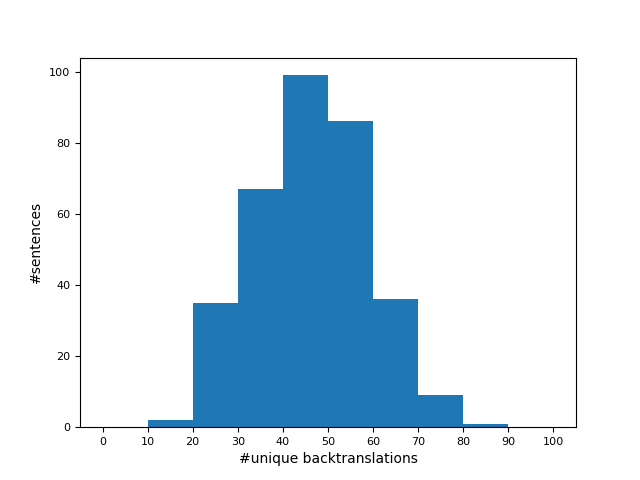
\includegraphics[width=\textwidth]{figures/unique_back_original.png}
         \caption{$y=5/x$}
         \label{fig:five over x}
     \end{subfigure}
        \caption{Three simple graphs}
        \label{fig:three graphs}

\end{figure}